\subsection{Définir des standards typologiques}

\begin{frame}
\frametitle{\darkhighlightiii{Introduction: comparaison de systèmes linguistiques}}
%\pause
\begin{wideitemize}
\item Enjeux généraux en typologie linguistique
\begin{smallwideitemize}
  \item décrire des propriétés partagées par des systèmes
  \item {décrire les différences entre ces systèmes}
  \item développer le vocabulaire adéquat pour les caractériser
\end{smallwideitemize}
%\item Canonical typology in particular
%\pause
\item {Emploi de standards comparatifs}
%\pause
\begin{smallwideitemize}
\item Il existe plusieurs critères possibles parmi lesquels:
\begin{smallwideitemize}\footnotesize
  \item prototypicité, dérivable d'universaux linguistiques \cite{greenberg63}
  \item naturalité \cite{wurzel84,dressler00}
  \item {canonicité \cite{corbett03,corbett07b}}
\end{smallwideitemize}
\end{smallwideitemize}
% \pause
% \item \highlightii{\parsli}
% \begin{smallwideitemize}
% \item \highlightii{a formal approach to typology} w.r.t inflectional morphology.
% \item Development of measures for quantitave typological evaluation of
%   morphological systems.
% \end{smallwideitemize}
%\pause
\invisibletext{
\item[] {Canonicité --- approche autonome reposant sur un système
    d'ontologies}
\begin{smallwideitemize}
\invisibletext{
  \item[] la définition du canon repose sur des \invisibletext{propriétés définitoires}
  \item[] il est défini par un \invisibletext{espace multidimensionnel} des possibles
  \item[] il permet de comparer chaque système individuel en
    termes de \invisibletext{déviation plus ou moins marquée par rapport à un
      \invisibletext{étalon canonique}}
}
\end{smallwideitemize}
}
%\pause
%\item here: \highlighti{Canonical Inflection}
\end{wideitemize}
\end{frame}

\begin{frame}[t]{Qualifier la différence}
\begin{center}
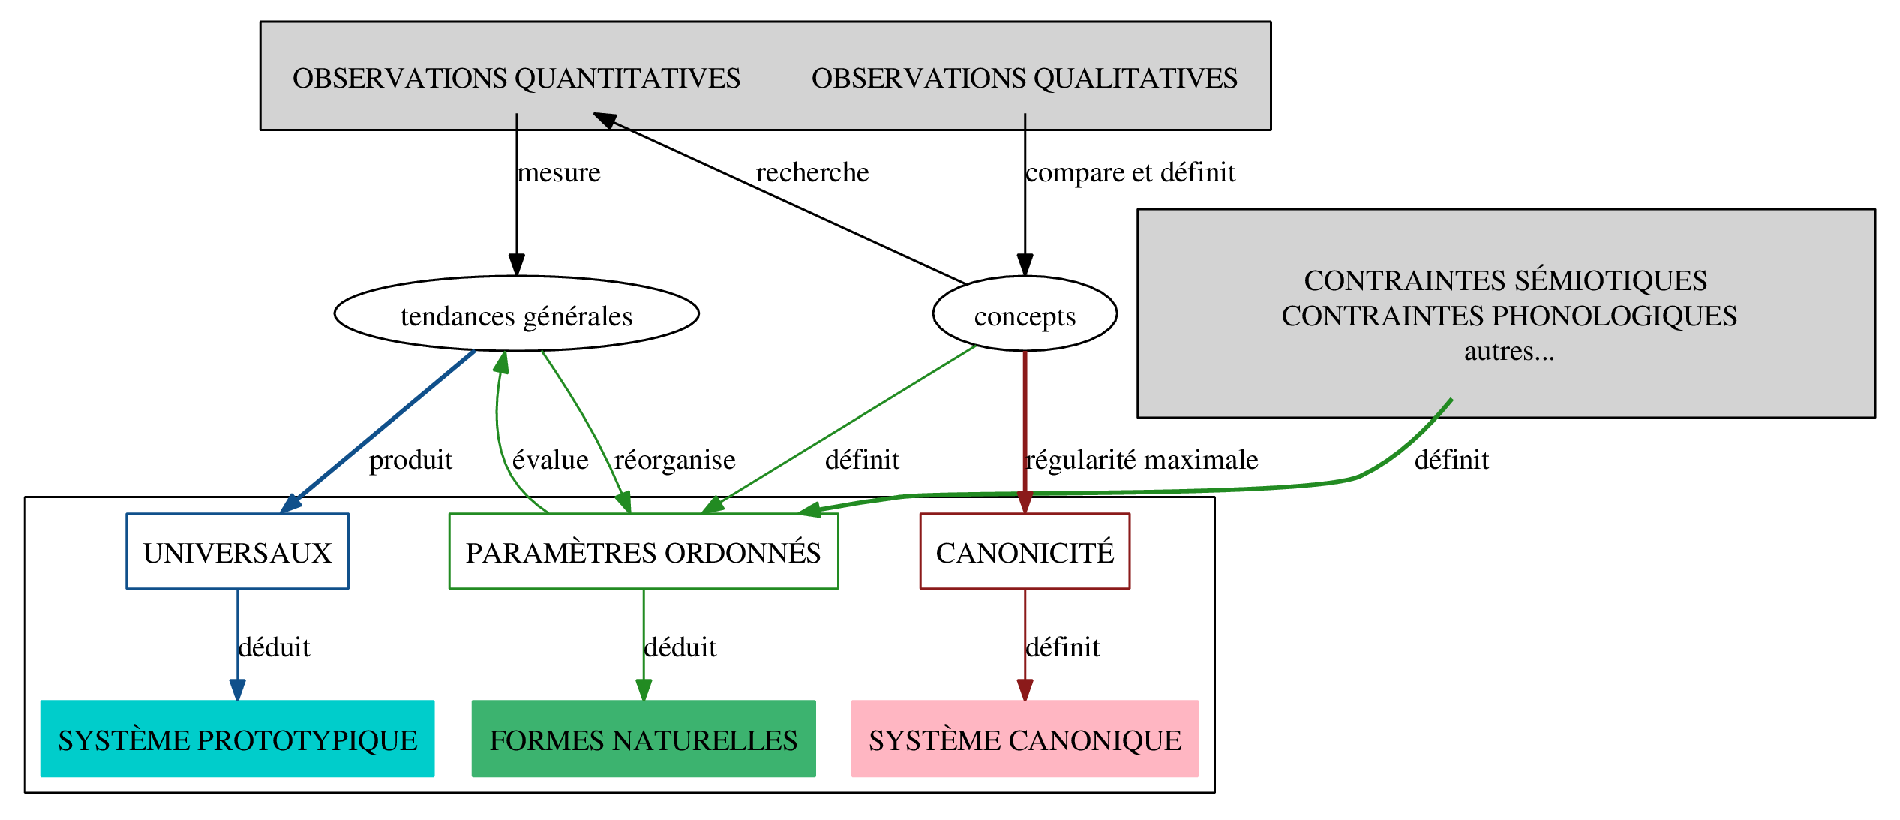
\includegraphics[width=120mm]{protonatcanon}
%\caption{Latin inflection zones}
\label{fig:canonicity}
\end{center}
\end{frame}

\begin{frame}
\frametitle{\darkhighlightiii{Comparaison de systèmes morphologiques}}
%\pause
\begin{wideitemize}
\item {Enjeux généraux en typologie linguistique}
\begin{smallwideitemize}
  \item {décrire des propriétés partagées par des systèmes}
  \item {décrire les différences entre ces systèmes}
  \item {développer le vocabulaire adéquat pour les caractériser}
\end{smallwideitemize}
%\item Canonical typology in particular
%\pause
\item {Emploi de standards comparatifs}
%\pause
\begin{smallwideitemize}
\item {Il existe plusieurs critères possibles parmi lesquels:}
\begin{smallwideitemize}
  \item {prototypes dérivables d'universaux linguistiques \cite{greenberg63}}
  \item {naturalité \cite{wurzel84,dressler00}}
  \item {canonicité \cite{corbett03,corbett07b}}
\end{smallwideitemize}
\end{smallwideitemize}
\pause
% \item \highlightii{\parsli}
% \begin{smallwideitemize}
% \item \highlightii{a formal approach to typology} w.r.t inflectional morphology.
% \item Development of measures for quantitave typological evaluation of
%   morphological systems.
% \end{smallwideitemize}
%\pause
\item Canonicité {\small --- approche autonome reposant sur un système
    d'ontologies}
\begin{smallwideitemize}
  \item la définition du canon repose sur des \lighthighlightiii{propriétés définitoires}
  \item il est défini par un \lighthighlightiii{espace multidimensionnel} des possibles
  \item il permet de comparer chaque système individuel en
    termes de \lighthighlightiii{déviation plus ou moins marquée par rapport à un
      \lighthighlightiii{étalon canonique}}
\end{smallwideitemize}
%\pause
%\item here: \highlighti{Canonical Inflection}
\end{wideitemize}
\end{frame}


\begin{frame}[t]{Représentation du canon selon Corbett {\em et al.} (2012) \nocite{corbett12imm}}
\begin{center}
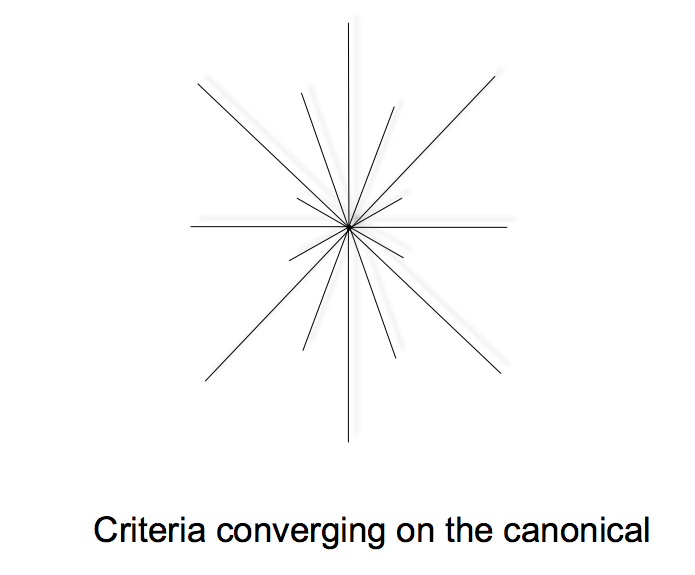
\includegraphics[width=80mm]{corbett-canon-star}
%\caption{Latin inflection zones}
\label{fig:canonicity}
\end{center}
\end{frame}


\begin{frame}
\frametitle{La typologie canonique}
\begin{wideitemize}
\item Concept de {\em typologie canonique}: \cite{corbett03}.
\item Différence entre un état hypothétique, idéal (c'est-à dire {\em
    canonique}) et les phénomènes réels qui sont observables.
\item {\em Flexion
  canonique} $\neq${\em  flexion prototypique}:
\begin{smallwideitemize}
%\item Canonical inflection is rare.
\item La flexion canonique correspond à un état idéal;
\item Elle constitue un espace théorique depuis lequel on peut mesurer
  les écarts observables,~\cite{corbett07b}.
\item Pour la comparaison entre les langues (notion typologique).
\end{smallwideitemize}
\item Quelques phénomènes non-canoniques:
\begin{smallwideitemize}
\item {\em supplétion} \cite{boye06,bonami06},
\item {\em déponence} \cite{baerman07bookdepo}, 
\item {\em hétéroclise} \cite{stump06a},
\item {\em
  défectivité} \cite{baerman10defectbook}
\item et plus récemment {\em
  surabondance} \cite{thornton10}.
\end{smallwideitemize}
\end{wideitemize}
\end{frame}

\subsection{La flexion canonique}


\begin{frame}
\frametitle{La flexion canonique}
La flexion canonique se définit par la comparaison des cases dans le
paradigme d'un lexème donné et par comparaison des paradigmes de
différents lexèmes entre eux.\\
Les cases sont censées avoir la même structure.

\scriptsize

\begin{table}
%\end{wideitemize}
\begin{tabular}{|l| p{1mm}|ll|p{1mm}|ll|p{1mm}cl}
\cline{1-1}\cline{3-4}\cline{6-7}
Traits&&\multicolumn{2}{|c|}{\textsc{ lexème~1}}&&\multicolumn{2}{|c|}{\textsc{ lexème~2}}&&\\
\cline{1-1}\cline{3-4}\cline{6-7}
\textsc{1.sg}&& radical1& {\em --ma}&&radical2& {\em
  --ma}&&\cellcolor{ciel}~~~&identique\\
\cline{1-1}\cline{3-4}\cline{6-7}
\textsc{2.sg}& &radical1&{\em --sa}&&radical2& {\em --sa}&&&\\
\cline{1-1}\cline{3-4}\cline{6-7}

\textsc{3.sg}&& radical1&{\em --ta}&&radical2& {\em
  --ta}&&\cellcolor{mandarine}&différent\\
\cline{1-1}\cline{3-4}\cline{6-7}
\textsc{1.pl}&&radical1& {\em --mo}&&radical2& {\em --mo}&&\\
\cline{1-1}\cline{3-4}\cline{6-7}
\textsc{2.pl}&&radical1& {\em --so}&&radical2& {\em --so}&&\\
\cline{1-1}\cline{3-4}\cline{6-7}
\textsc{3.pl}&&radical1& {\em --to}&&radical2& {\em --to}&&\\
\cline{1-1}\cline{3-4}\cline{6-7}
\end{tabular}\\[1mm]
\end{table}
\end{frame}

\iffalse
\begin{frame}
\frametitle{Canonical Inflection: criteria from \cite{corbett07b}}
\begin{table}\centering
\scalebox{0.88}{
\noindent\begin{tabular}{lp{4cm}@{~~~}l@{~~~}l}
\hline
&&\textsc{ comparison across }&\textsc{
  comparison }\\
&&\textsc{ cells of a lexème}&\textsc{
  across lexèmes}\\
\hline
1~~~&\textsc{ composition/structure} & {\em identique}& {\em identique}\\[1em]
2~~~&\textsc{ matériau lexical}  ($\approx$~apparence du radical) & {\em identique}& {\em différent}\\[1em]
3~~~&\textsc{ matériau flexionnel} ($\approx$~apparence des marques flex.)& {\em différent}& {\em identique}\\[1em]
4~~~&\textsc{ forme produite}  ($\approx$~apparence du mot-forme)& {\em différent}& {\em différent}\\[1em]\hline
&\\[-6pt]
\end{tabular}
}
\caption{La flexion canonique selon\cite{corbett07b}.}
\label{tbl:canonical-infl-corbett}
\end{table}
\end{frame}
\fi

\begin{frame}
\frametitle{Flexion canonique}
Comparaison des cases d'un paradigme donné.

\scriptsize

\begin{table}
%\end{wideitemize}
\begin{tabular}{|l| p{1mm}|ll|p{1mm}|ll|p{1mm}cl}
\cline{1-1}\cline{3-4}\cline{6-7}
Traits&&\multicolumn{2}{|c|}{\cellcolor{white}\textsc{ lexème~1}}&&\multicolumn{2}{|c|}{\textsc{ lexème~2}}&&\\
\cline{1-1}\cline{3-4}\cline{6-7}
\textsc{1.sg}&& \cellcolor{ciel}radical1& {\em --ma}&&radical2& {\em
  --ma}&&\cellcolor{ciel}~~~&identique\\
\cline{1-1}\cline{3-4}\cline{6-7}
\textsc{2.sg}& &radical1&{\em --sa}&&radical2& {\em --sa}&&&\\
\cline{1-1}\cline{3-4}\cline{6-7}

\textsc{3.sg}&& radical1&{\em --ta}&&radical2& {\em
  --ta}&&\cellcolor{mandarine}&différent\\
\cline{1-1}\cline{3-4}\cline{6-7}
\textsc{1.pl}&&radical1& {\em --mo}&&radical2& {\em --mo}&&\\
\cline{1-1}\cline{3-4}\cline{6-7}
\textsc{2.pl}&&radical1& {\em --so}&&radical2& {\em --so}&&\\
\cline{1-1}\cline{3-4}\cline{6-7}
\textsc{3.pl}&&radical1& {\em --to}&&radical2& {\em --to}&&\\
\cline{1-1}\cline{3-4}\cline{6-7}
\end{tabular}\\[1mm]
\end{table}
\end{frame}

\begin{frame}
\frametitle{Flexion canonique}
Comparaison des cases d'un paradigme donné.

\scriptsize

\begin{table}
%\end{wideitemize}
\begin{tabular}{|l| p{1mm}|ll|p{1mm}|ll|p{1mm}cl}
\cline{1-1}\cline{3-4}\cline{6-7}
Traits&&\multicolumn{2}{|c|}{\cellcolor{white}\textsc{ lexème~1}}&&\multicolumn{2}{|c|}{\textsc{ lexème~2}}&&\\
\cline{1-1}\cline{3-4}\cline{6-7}
\textsc{1.sg}&& \cellcolor{ciel}radical1& {\em --ma}&&radical2& {\em
  --ma}&&\cellcolor{ciel}~~~&identique\\
\cline{1-1}\cline{3-4}\cline{6-7}
\textsc{2.sg}& &\cellcolor{ciel}radical1&{\em --sa}&&radical2& {\em --sa}&&&\\
\cline{1-1}\cline{3-4}\cline{6-7}

\textsc{3.sg}&& \cellcolor{ciel}radical1&{\em --ta}&&radical2& {\em
  --ta}&&\cellcolor{mandarine}&différent\\
\cline{1-1}\cline{3-4}\cline{6-7}
\textsc{1.pl}&&\cellcolor{ciel}radical1& {\em --mo}&&radical2& {\em --mo}&&\\
\cline{1-1}\cline{3-4}\cline{6-7}
\textsc{2.pl}&&\cellcolor{ciel}radical1& {\em --so}&&radical2& {\em --so}&&\\
\cline{1-1}\cline{3-4}\cline{6-7}
\textsc{3.pl}&&\cellcolor{ciel}radical1& {\em --to}&&radical2& {\em --to}&&\\
\cline{1-1}\cline{3-4}\cline{6-7}
\end{tabular}\\[1mm]
\end{table}
\end{frame}

\begin{frame}
\frametitle{Flexion canonique}
Comparaison des cases d'un paradigme donné.

\scriptsize

\begin{table}
%\end{wideitemize}
\begin{tabular}{|l| p{1mm}|ll|p{1mm}|ll|p{1mm}cl}
\cline{1-1}\cline{3-4}\cline{6-7}
Traits&&\multicolumn{2}{|c|}{\cellcolor{white}\textsc{ lexème~1}}&&\multicolumn{2}{|c|}{\textsc{ lexème~2}}&&\\
\cline{1-1}\cline{3-4}\cline{6-7}
\textsc{1.sg}&& \cellcolor{ciel}radical1& \cellcolor{mandarine}{\em --ma}&&radical2& {\em
  --ma}&&\cellcolor{ciel}~~~&identique\\
\cline{1-1}\cline{3-4}\cline{6-7}
\textsc{2.sg}& &\cellcolor{ciel}radical1&{\em --sa}&&radical2& {\em --sa}&&&\\
\cline{1-1}\cline{3-4}\cline{6-7}

\textsc{3.sg}&& \cellcolor{ciel}radical1&{\em --ta}&&radical2& {\em
  --ta}&&\cellcolor{mandarine}&différent\\
\cline{1-1}\cline{3-4}\cline{6-7}
\textsc{1.pl}&&\cellcolor{ciel}radical1& {\em --mo}&&radical2& {\em --mo}&&\\
\cline{1-1}\cline{3-4}\cline{6-7}
\textsc{2.pl}&&\cellcolor{ciel}radical1& {\em --so}&&radical2& {\em --so}&&\\
\cline{1-1}\cline{3-4}\cline{6-7}
\textsc{3.pl}&&\cellcolor{ciel}radical1& {\em --to}&&radical2& {\em --to}&&\\
\cline{1-1}\cline{3-4}\cline{6-7}
\end{tabular}\\[1mm]
\end{table}
\end{frame}

\begin{frame}
%\frametitle{Canonical Inflection}
\frametitle{Flexion canonique}
Comparaison des cases d'un paradigme donné.

\scriptsize

\begin{table}
%\end{wideitemize}
\begin{tabular}{|l| p{1mm}|ll|p{1mm}|ll|p{1mm}cl}
\cline{1-1}\cline{3-4}\cline{6-7}
Traits&&\multicolumn{2}{|c|}{\cellcolor{white}\textsc{ lexème~1}}&&\multicolumn{2}{|c|}{\textsc{ lexème~2}}&&\\
\cline{1-1}\cline{3-4}\cline{6-7}
\textsc{1.sg}&& \cellcolor{ciel}radical1& \cellcolor{mandarine}{\em --ma}&&radical2& {\em
  --ma}&&\cellcolor{ciel}~~~&identique\\
\cline{1-1}\cline{3-4}\cline{6-7}
\textsc{2.sg}& &\cellcolor{ciel}radical1&\cellcolor{mandarine}{\em --sa}&&radical2& {\em --sa}&&&\\
\cline{1-1}\cline{3-4}\cline{6-7}

\textsc{3.sg}&& \cellcolor{ciel}radical1&\cellcolor{mandarine}{\em --ta}&&radical2& {\em
  --ta}&&\cellcolor{mandarine}&différent\\
\cline{1-1}\cline{3-4}\cline{6-7}
\textsc{1.pl}&&\cellcolor{ciel}radical1& \cellcolor{mandarine}{\em --mo}&&radical2& {\em --mo}&&\\
\cline{1-1}\cline{3-4}\cline{6-7}
\textsc{2.pl}&&\cellcolor{ciel}radical1& \cellcolor{mandarine}{\em --so}&&radical2& {\em --so}&&\\
\cline{1-1}\cline{3-4}\cline{6-7}
\textsc{3.pl}&&\cellcolor{ciel}radical1& \cellcolor{mandarine}{\em --to}&&radical2& {\em --to}&&\\
\cline{1-1}\cline{3-4}\cline{6-7}
\end{tabular}\\[1mm]
\end{table}
\end{frame}

\begin{frame}
\frametitle{Flexion canonique}
Comparaison des cases d'un paradigme à l'autre.

\scriptsize

\begin{table}
%\end{wideitemize}
\begin{tabular}{|l| p{1mm}|ll|p{1mm}|ll|p{1mm}cl}
\cline{1-1}\cline{3-4}\cline{6-7}
Traits&&\multicolumn{2}{|c|}{\cellcolor{white}\textsc{ lexème~1}}&&\multicolumn{2}{|c|}{\cellcolor{white}\textsc{ lexème~2}}&&\\
\cline{1-1}\cline{3-4}\cline{6-7}
\textsc{1.sg}&& radical1& {\em --ma}&&radical2& {\em
  --ma}&&\cellcolor{ciel}~~~&identique\\
\cline{1-1}\cline{3-4}\cline{6-7}
\textsc{2.sg}& &radical1&{\em --sa}&&radical2& {\em --sa}&&&\\
\cline{1-1}\cline{3-4}\cline{6-7}

\textsc{3.sg}&& radical1&{\em --ta}&&radical2& {\em
  --ta}&&\cellcolor{mandarine}&différent\\
\cline{1-1}\cline{3-4}\cline{6-7}
\textsc{1.pl}&&radical1& {\em --mo}&&radical2& {\em --mo}&&\\
\cline{1-1}\cline{3-4}\cline{6-7}
\textsc{2.pl}&&radical1& {\em --so}&&radical2& {\em --so}&&\\
\cline{1-1}\cline{3-4}\cline{6-7}
\textsc{3.pl}&&radical1& {\em --to}&&radical2& {\em --to}&&\\
\cline{1-1}\cline{3-4}\cline{6-7}
\end{tabular}\\[1mm]
\end{table}
\end{frame}

\begin{frame}
\frametitle{Flexion canonique}
Comparaison des cases d'un paradigme à l'autre.

\scriptsize

\begin{table}
%\end{wideitemize}
\begin{tabular}{|l| p{1mm}|ll|p{1mm}|ll|p{1mm}cl}
\cline{1-1}\cline{3-4}\cline{6-7}
Traits&&\multicolumn{2}{|c|}{\cellcolor{white}\textsc{ lexème~1}}&&\multicolumn{2}{|c|}{\cellcolor{white}\textsc{ lexème~2}}&&\\
\cline{1-1}\cline{3-4}\cline{6-7}
\textsc{1.sg}&& \cellcolor{mandarine}radical1& \cellcolor{ciel}{\em --ma}&&\cellcolor{mandarine}radical2& \cellcolor{ciel}{\em
  --ma}&&\cellcolor{ciel}~~~&identique\\
\cline{1-1}\cline{3-4}\cline{6-7}
\textsc{2.sg}& &radical1&{\em --sa}&&radical2& {\em --sa}&&&\\
\cline{1-1}\cline{3-4}\cline{6-7}

\textsc{3.sg}&& radical1&{\em --ta}&&radical2& {\em
  --ta}&&\cellcolor{mandarine}&différent\\
\cline{1-1}\cline{3-4}\cline{6-7}
\textsc{1.pl}&&radical1& {\em --mo}&&radical2& {\em --mo}&&\\
\cline{1-1}\cline{3-4}\cline{6-7}
\textsc{2.pl}&&radical1& {\em --so}&&radical2& {\em --so}&&\\
\cline{1-1}\cline{3-4}\cline{6-7}
\textsc{3.pl}&&radical1& {\em --to}&&radical2& {\em --to}&&\\
\cline{1-1}\cline{3-4}\cline{6-7}
\end{tabular}\\[1mm]
\end{table}
\end{frame}


\begin{frame}
\frametitle{Flexion canonique}
Comparaison des cases d'un paradigme à l'autre.

\scriptsize

\begin{table}
%\end{wideitemize}
\begin{tabular}{|l| p{1mm}|ll|p{1mm}|ll|p{1mm}cl}
\cline{1-1}\cline{3-4}\cline{6-7}
Traits&&\multicolumn{2}{|c|}{\cellcolor{white}\textsc{ lexème~1}}&&\multicolumn{2}{|c|}{\cellcolor{white}\textsc{ lexème~2}}&&\\
\cline{1-1}\cline{3-4}\cline{6-7}
\textsc{1.sg}&& \cellcolor{mandarine}radical1& {\em --ma}&&\cellcolor{mandarine}radical2& {\em
  --ma}&&\cellcolor{ciel}~~~&identique\\
\cline{1-1}\cline{3-4}\cline{6-7}
\textsc{2.sg}& &radical1&\cellcolor{ciel}{\em --sa}&&radical2&\cellcolor{ciel} {\em --sa}&&&\\
\cline{1-1}\cline{3-4}\cline{6-7}
\textsc{3.sg}&& radical1&{\em --ta}&&radical2& {\em
  --ta}&&\cellcolor{mandarine}&différent\\
\cline{1-1}\cline{3-4}\cline{6-7}
\textsc{1.pl}&&radical1& {\em --mo}&&radical2& {\em --mo}&&\\
\cline{1-1}\cline{3-4}\cline{6-7}
\textsc{2.pl}&&radical1& {\em --so}&&radical2& {\em --so}&&\\
\cline{1-1}\cline{3-4}\cline{6-7}
\textsc{3.pl}&&radical1& {\em --to}&&radical2& {\em --to}&&\\
\cline{1-1}\cline{3-4}\cline{6-7}
\end{tabular}\\[1mm]
\end{table}
\end{frame}


\begin{frame}
\frametitle{Flexion canonique}
Comparaison des cases d'un paradigme à l'autre.

\scriptsize

\begin{table}
%\end{wideitemize}
\begin{tabular}{|l| p{1mm}|ll|p{1mm}|ll|p{1mm}cl}
\cline{1-1}\cline{3-4}\cline{6-7}
Traits&&\multicolumn{2}{|c|}{\cellcolor{white}\textsc{ lexème~1}}&&\multicolumn{2}{|c|}{\cellcolor{white}\textsc{ lexème~2}}&&\\
\cline{1-1}\cline{3-4}\cline{6-7}
\textsc{1.sg}&& \cellcolor{mandarine}radical1& {\em --ma}&&\cellcolor{mandarine}radical2& {\em
  --ma}&&\cellcolor{ciel}~~~&identique\\
\cline{1-1}\cline{3-4}\cline{6-7}
\textsc{2.sg}& &radical1&{\em --sa}&&radical2& {\em --sa}&&&\\
\cline{1-1}\cline{3-4}\cline{6-7}

\textsc{3.sg}&& radical1&\cellcolor{ciel}{\em --ta}&&radical2& \cellcolor{ciel}{\em
  --ta}&&\cellcolor{mandarine}&différent\\
\cline{1-1}\cline{3-4}\cline{6-7}
\textsc{1.pl}&&radical1&\cellcolor{ciel}{\em --mo}&&radical2&\cellcolor{ciel}{\em --mo}&&\\
\cline{1-1}\cline{3-4}\cline{6-7}
\textsc{2.pl}&&radical1& \cellcolor{ciel}{\em --so}&&radical2&\cellcolor{ciel}{\em --so}&&\\
\cline{1-1}\cline{3-4}\cline{6-7}
\textsc{3.pl}&&radical1&\cellcolor{ciel}{\em --to}&&radical2&\cellcolor{ciel}{\em --to}&&\\
\cline{1-1}\cline{3-4}\cline{6-7}
\end{tabular}\\[1mm]
\end{table}
\end{frame}


\begin{frame}
\frametitle{Flexion canonique}
\begin{itemize}
\item toutes les formes sont différentes les unes des autres;
\item il y a exactement une forme (unique) qui exprime une structure
  de traits morphosyntaxiques donnée ($\approx$ une case= une forme phonologique/graphémique).
\end{itemize}

\scriptsize
\begin{table}
%\end{wideitemize}
\begin{tabular}{|l| p{1mm}|ll|p{1mm}|ll|p{1mm}cl}
\cline{1-1}\cline{3-4}\cline{6-7}
Traits&&\multicolumn{2}{|c|}{\cellcolor{white}\textsc{ lexème~1}}&&\multicolumn{2}{|c|}{\cellcolor{white}\textsc{ lexème~2}}&&\\
\cline{1-1}\cline{3-4}\cline{6-7}
\textsc{1.sg}&& \cellcolor{mandarine}radical1&\cellcolor{mandarine}{\em --ma}&&\cellcolor{mandarine}radical2&\cellcolor{mandarine}{\em
  --ma}&&\cellcolor{ciel}~~~&identique\\
\cline{1-1}\cline{3-4}\cline{6-7}
\textsc{2.sg}& &\cellcolor{mandarine}radical1&\cellcolor{mandarine}{\em --sa}&&\cellcolor{mandarine}radical2&\cellcolor{mandarine}{\em --sa}&&&\\
\cline{1-1}\cline{3-4}\cline{6-7}
\textsc{3.sg}&& \cellcolor{mandarine}radical1&\cellcolor{mandarine}{\em --ta}&&\cellcolor{mandarine}radical2& \cellcolor{mandarine}{\em
  --ta}&&\cellcolor{mandarine}&différent\\
\cline{1-1}\cline{3-4}\cline{6-7}
\textsc{1.pl}&&\cellcolor{mandarine}radical1&\cellcolor{mandarine}{\em --mo}&&\cellcolor{mandarine}radical2&\cellcolor{mandarine}{\em --mo}&&\\
\cline{1-1}\cline{3-4}\cline{6-7}
\textsc{2.pl}&&\cellcolor{mandarine}radical1&\cellcolor{mandarine}{\em --so}&&\cellcolor{mandarine}radical2&\cellcolor{mandarine}{\em --so}&&\\
\cline{1-1}\cline{3-4}\cline{6-7}
\textsc{3.pl}&&\cellcolor{mandarine}radical1& \cellcolor{mandarine}{\em
  --to}&&\cellcolor{mandarine}radical2&\cellcolor{mandarine}{\em --to}&&\\
\cline{1-1}\cline{3-4}\cline{6-7}
\end{tabular}\\[1mm]
\end{table}
\end{frame}


\subsection{Les phénomènes non-canoniques}

\begin{frame}
\frametitle{Phénomènes non-canoniques}
\begin{wideitemize}
\item Une fois cette régularité maximale définie, on peut définir des
  déviations pour chacune des dimensions qui la constituent
\item Méthode qui permet un typage explicite des déviations\\
\ra~ par rapport à la réalisation des formes\\
\ra~ par rapport au remplissage des
cases du paradigme\\
\ra~ dans la définition des traits morphosyntaxiques exprimés\\
\end{wideitemize}
\end{frame}


%%%%formes
\begin{frame}
\frametitle{Irrégularité dans les formes}
\framesubtitle{Syncrétismes (latin)}
\begin{center}
\begin{tabular}{l|ll|ll}
&\multicolumn{2}{c|}{\scriptsize{FILIUS}
  'fils'}&\multicolumn{2}{c}{\scriptsize{BELLUM} 'guerre'}\\
&{\scriptsize{SG}}&{\scriptsize{PL}}&{\scriptsize{SG}}&{\scriptsize{PL}}\\
\hline
{\scriptsize{NOM}}&fili-us&fili\highlightiv{-i}&bell-\highlighti{um}&bell\highlightii{-a}\\
{\scriptsize{VOC}}&fili-e&fili\highlightiv{-i}&(bell-\highlighti{um})&(bell\highlightii{-a})\\
{\scriptsize{ACC}}&fili-um&fili-\=os&bell\highlighti{-um}&bell\highlightii{-a}\\
{\scriptsize{GEN}}&fili\highlightiv{-i}&fili-\=orum&bell-i&bell-\=orum\\
{\scriptsize{DAT}}&fili\highlightiii{-\=o}&fili\highlightii{-\=is}&bell\highlightiii{-o}&bell-\highlightiv{\=is}\\
{\scriptsize{ABL}}&fili\highlightiii{-\=o}&fili\highlightii{-\=is}&bell\highlightiii{-o}&bell-\highlightiv{\=is}\\
\end{tabular}
\end{center}
\end{frame}

\begin{frame}
\frametitle{Irrégularité dans les formes}
\framesubtitle{Classes flexionnelles (latin)}
\begin{center}
\begin{tabular}{l|ll|ll}
&\multicolumn{2}{c|}{\scriptsize{FILIUS}
  'fils'}&\multicolumn{2}{c}{\scriptsize{AGRICOLA} 'paysan'}\\
&{\scriptsize{SG}}&{\scriptsize{PL}}&{\scriptsize{SG}}&{\scriptsize{PL}}\\
\hline
{\scriptsize{NOM}}&fili-us&fili\highlightiv{-i}&agricol-\highlighti{a}&agricol\highlightiii{-ae}\\
{\scriptsize{VOC}}&fili-e&fili\highlightiv{-i}&agricol-\highlighti{a}&agricol\highlightiii{-ae}\\
{\scriptsize{ACC}}&fili-um&fili-\=os&agricol{-am}&agricol{-\=as}\\
{\scriptsize{GEN}}&fili\highlightiv{-i}&fili-\=orum&agricol\highlightiii{-ae}&agricol-\=arum\\
{\scriptsize{DAT}}&fili\highlightiii{-\=o}&fili\highlightii{-\=is}&agricol\highlightiii{-ae}&agricol-\highlightiv{\=is}\\
{\scriptsize{ABL}}&fili\highlightiii{-\=o}&fili\highlightii{-\=is}&agricol-\=a&agricol-\highlightiv{\=is}\\
\end{tabular}
\end{center}
\end{frame}





\begin{frame}
\frametitle{Irrégularité dans les formes}
\framesubtitle{Supplétion}
\begin{description}
\item[{\bf Allomorphie}] Changement de radical, souvent conditionné phonologiquement.
\item[{\bf Supplétion de radical}] Allomorphie irrégulière extrème.
\end{description}
\end{frame}



\begin{frame}
\frametitle{Irrégularité dans les formes}
\framesubtitle{Supplétion}
\begin{wideitemize}
\item Il y a deux types de supplétion: la {\em supplétion de radical}
  et la {\em suppletion de forme} \cite{boye06}.
\item Supplétion de radical: à l'intérieur du paradigme les formes
  restent régulières et les exposants sont reconnaissables.
\item Supplétion de forme: une forme complète a été insérée dans le
  paradigme --- la forme canonique n'existe pas.
\end{wideitemize}
\end{frame}


\begin{frame}
\frametitle{Irrégularité dans les formes}
\framesubtitle{Supplétion selon \cite{boye06}}
%\pause
Supplétion de radicaux:  à l'interieur d'un paradigme; les formes à
l'intérieur d'un paradigmes sont régulières; on reconnait l'exposant.

\scriptsize
\begin{table}
\begin{tabular}{|l|p{1mm}|ll|p{1mm}|ll|p{1mm}cl}
\cline{1-1}\cline{3-4}\cline{6-7}
Traits&&\multicolumn{2}{|c|}{\scriptsize{CHANTER}}&&\multicolumn{2}{|c|}{\scriptsize{ALLER}}&&\\
\cline{1-1}\cline{3-4}\cline{6-7}
\textsc{1.sg}&& chant& {\em --e}&&v& {\em
  --ais}&&\cellcolor{ciel}~~~&régulier\\
\cline{1-1}\cline{3-4}\cline{6-7}
\textsc{2.sg} &&chant&{\em --es}&&v& {\em --as}&&&\\
\cline{1-1}\cline{3-4}\cline{6-7}
\textsc{3.sg}&& chant&{\em --e}&&v& {\em
  --a}&&\cellcolor{mandarine}&supplétif\\
\cline{1-1}\cline{3-4}\cline{6-7}
\textsc{1.pl}&&chant&\cellcolor{ciel}{\em --ons}&&\cellcolor{mandarine} all& \cellcolor{ciel}{\em --ons}&&\\
\cline{1-1}\cline{3-4}\cline{6-7}
\textsc{2.pl}&&chant& \cellcolor{ciel}{\em --ez}&&\cellcolor{mandarine} all& \cellcolor{ciel}{\em --ez}&&\\
\cline{1-1}\cline{3-4}\cline{6-7}
\textsc{3.pl}&&chant& {\em --ent}&&v& {\em --ont}&&\\
\cline{1-1}\cline{3-4}\cline{6-7}
\end{tabular}\\[1mm]
\end{table}
\end{frame}


\begin{frame}
\frametitle{Irrégularité dans les formes}
\framesubtitle{Supplétion de forme \cite{boye06}}
Supplétion de forme: une forme complète est insérée dans le paradigme
et bloque ainsi la rélisation d'autres règles.

\begin{table}
\begin{tabular}{|l| p{1mm}|ll|p{1mm}|ll|p{1mm}cl}
\cline{1-1}\cline{3-4}\cline{6-7}
Traits&&\multicolumn{2}{|c|}{\scriptsize{CHANTER}}&&\multicolumn{2}{|c|}{\scriptsize{ÊTRE}}&&\\
\cline{1-1}\cline{3-4}\cline{6-7}
\textsc{1.pl}&&chant& {\em --ons}&&\multicolumn{2}{|l|}{\cellcolor{mandarine} sommes}& {\em }&&\\
\cline{1-1}\cline{3-4}\cline{6-7}
\end{tabular}\\[1mm]
\end{table}
\end{frame}


%%%%%%%cases




\begin{frame}
\frametitle{Irrégularité dans le remplissage des cases}
\framesubtitle{Défectivité}
\vspace{2ex}
Un exemple de défectivité est celui des {\em pluralia tantum}
pour lesquels il n'existe que des formes du pluriel.
\begin{itemize}
\item {\scriptsize{VIVRES}} en français,
\item {\scriptsize{TROUSERS}} 'pantalon' en anglais,
\item ou encore {\scriptsize{VIANOCE}} 'Noël' en slovaque.
\end{itemize}

\vspace{2ex}

\footnotesize
\begin{tabular}{lll}
&{\scriptsize{SG}}&{\scriptsize{PL}}\\
\hline
{\scriptsize{VIVRES}}&\cellcolor{black}&{\em vivres}\\[1ex]
{\scriptsize{TROUSERS}}&\cellcolor{black}&{\em trousers}\\[1ex]
{\scriptsize{VIANOCE}}&\cellcolor{black}&{\em Vianoce}\\[1ex]
\end{tabular}


\end{frame}




\begin{frame}
\frametitle{Irrégularité dans le remplissage des cases}
\framesubtitle{Surabondance}
La contre-partie évidente à la défectivité est la notion de {\em
  surabondance}. 
\begin{itemize}
\item On parle de {\em surabondance} à chaque fois qu'une
case d'un paradigme donné contient plus d'une forme.
\item La notion de
surabondance a été introduite par \cite{thornton10} pour
l'italien.
\item Deux formes: {\em cell-mates} (en), {\em compagni di cella} (it),{\em
    ``compagnons de cellule''?} (fr).
\end{itemize}

\pause
\begin{table}\centering
\scalebox{0.9}{
\begin{tabular}{l@{~~~~}l@{~~~~}l}
\hline
\textsc{ }  & \textsc{ forme~1} & \textsc{ forme~2}\\
\hline
{'languir' \textsc{ 3pl.prs.subj}}& {\em languano}& {\em languiscano}\\
[1ex]
{'posséder' \textsc{ 3pl.prs.subj}}&  {\em possiedano}& {\em posseggano}\\
[1ex]
{'posséder' \textsc{ 3sg.prs.subj}}&  {\em possieda}& {\em possegga}\\
[1ex]
{'posséder' \textsc{ 1sg.prs.subj}}&  {\em possiedo}& {\em posseggo}\\
[2ex]
\end{tabular}
}
%\caption{surabondance en \cite{thornton10}}
\label{tbl:italian}
\end{table}
\end{frame}






%%%%%%traits

\begin{frame}

\frametitle{Irrégularité dans le l'expression des traits morphosyntaxiques}
\framesubtitle{Décalage morphosyntaxique ou déponence}
Les noms du serbo-croate emploient parfois des formes du singulier pour
exprimer le pluriel \cite{baerman06depoData}.

\vspace{2ex}
\begin{multicols}{2}
\scalebox{0.65}{\centering
\noindent
\begin{tabular}{l@{~~}l@{~}l@{~~}l@{~}l@{~~}l@{~}l}
\hline
&
\multicolumn{2}{c}{\textsc{ 
féminin à radical en --a}
}&
\multicolumn{2}{c}{\textsc{ 
féminin à radical en --i}
}\\
&\multicolumn{2}{c}{{\scriptsize{ŽENA}} 'femme'}
&
\multicolumn{2}{c}{{\scriptsize{STVAR}} 'chose'}\\
\hline
                 &\textsc{singulier  }&\textsc{pluriel}&\textsc{singulier}&\textsc{pluriel}\\
\textsc{nom }&\cellcolor{mandarine}{\em žen-a}&{\em žen-e}&\cellcolor{ciel}{\em stvar}&{\em stvar-i}\\
\textsc{acc }&\cellcolor{mandarine}{\em žen-u} & {\em žen-e}&\cellcolor{ciel}{\em stvar}&{\em stvar-i}\\
\textsc{gen} &\cellcolor{mandarine}{\em žen-e} & {\em žen-a}&\cellcolor{ciel}{\em stvar-i}&{\em stvar-i}\\
\textsc{dat }&\cellcolor{mandarine}{\em žen-i}&{\em žen-ama}&\cellcolor{ciel}{\em stvar-i}&{\em stvar-ima}\\
\textsc{ins} &\cellcolor{mandarine}{\em žen-om}&{\em žen-ama}&\cellcolor{ciel}{\em stvar-i}&{\em stvar-im}\\[2ex]
\end{tabular}
}

\scalebox{0.65}{
\begin{tabular}{|@{~~}l@{~}l@{~~}l@{~}l}
\hline
\multicolumn{2}{|c@{~~}}{\textsc{ neut. -et$\sim$a-stem}
}&
\multicolumn{2}{c}{\textsc{ 
neut. -et$\sim$i-stem}
}\\
\multicolumn{2}{|c}{
 {\scriptsize{DETE}}  'enfant'}
&\multicolumn{2}{c}{
 {\scriptsize{TELE}}  'veau'}
\\
\hline
\textsc{ singulier}&\textsc{ pluriel  }&\textsc{ singulier  }&\textsc{ pluriel  }\\
%\textsc{ nom }& 
{\em  dete}& \cellcolor{mandarine}{\em dec-a}  & {\em  tele}&\cellcolor{ciel}{\em telad}\\
%\textsc{ acc }& 
{\em  dete}& \cellcolor{mandarine}{\em dec-u} & {\em  tele}& \cellcolor{ciel}{\em telad}\\
%\textsc{ gen }& 
{\em  deteta}& \cellcolor{mandarine}{\em dec-e} & {\em  teleta}& {\em telad}\\
%\textsc{ dat }&
 {\em  detetu}& \cellcolor{mandarine}{\em dec-i} & {\em  teletu}& \cellcolor{ciel}{\em telad-i(ma)}\\
%\textsc{ ins }&
 {\em  detetom  }& \cellcolor{mandarine}{\em dec-om} & {\em  teletom  }& \cellcolor{ciel}{\em telad-i(ma)  }\\[2ex]
\end{tabular}
}
\end{multicols}

\end{frame}


%%%%%%%



\begin{frame}[t]{Phénomènes non-canoniques}
     \begin{columns}[t] % contents are top vertically aligned
     \begin{column}[T]{5cm} % each column can also be its own environment
\vspace*{-.5cm}
\begin{wideitemize}
\item \highlightiv{La typologie canonique en morphologie flexionnelle:}

\begin{smallwideitemize}\scriptsize
\item[\highlightii{+}] définition qualitative des différents types de déviation
  possibles par rapport au canon
\item[\highlightii{+}] notion de déviation plus ou moins importante selon les systèmes
% \end{smallwideitemize}

% % \item \highlightii{Objectif de la thèse:}

% % \begin{smallwideitemize}
% % \item[\highlightii{+}] formalisation de la définition de chaque phénomène
% % \item[\highlightii{+}] définition de mesures quantitatives
% % \end{smallwideitemize}
%  \end{wideitemize}

%      \end{column}
%      \begin{column}[T]{8cm} % alternative top-align that's better for
%                             % graphics
% %\vspace*{-4cm}
%           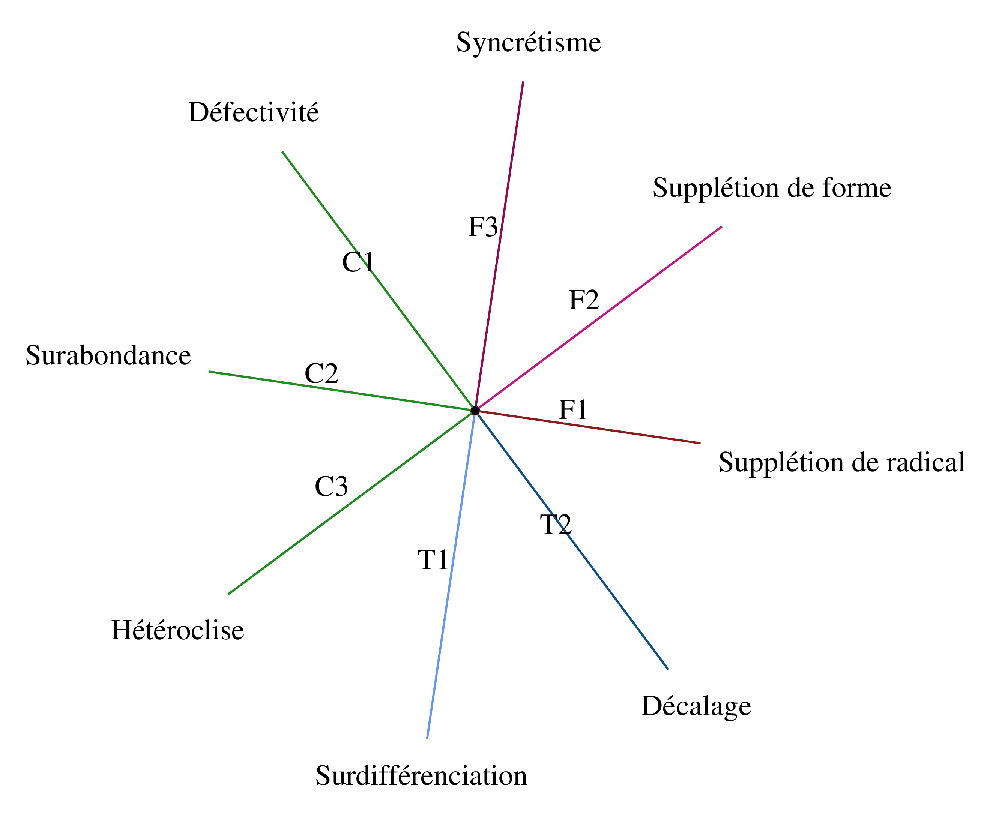
\includegraphics[height=6.5cm]{canonicity}
%      \end{column}
%      \end{columns}
% \end{frame}

% \begin{frame}[t]{Formalisation des phénomènes non-canoniques en \protect\parsli}
%      \begin{columns}[t] % contents are top vertically aligned
%      \begin{column}[T]{6cm} % each column can also be its own environment
% \vspace*{-.5cm}
% \begin{wideitemize}\footnotesize
% \item \highlightii{Formaliser la morphologie canonique:}

% \begin{smallwideitemize}\scriptsize
% \item[\highlightii{+}] définition formelle des différents types de déviation
%   possibles par rapport au canon
% \item[\highlightii{+}] raffinement de certaines définitions:\\
% \ra~allomorphie radicale/supplétion de radicaux
% \ra~défectivité/déficience
\item[\highlightii{+}] Classement possible des types de déviation:\\%\scriptsize
\ra~ dans la définition des traits: T1-T3\\
\ra~ des résultats: F1-F3\\
\ra~ dans la réalisation: C1-C4\\
\cite{walther13phd}
\end{smallwideitemize}

%\item \highlighti{Quantifier la morphologie canonique:}

% \begin{smallwideitemize}\scriptsize
% \item[\highlighti{+}] définition de mesures quantitatives des 10
%   déviations possibles par rapport au canon
% \end{smallwideitemize}

\end{wideitemize}

     \end{column}
     \begin{column}[T]{7cm} % alternative top-align that's better for
                            % graphics
%\vspace*{-4cm}
          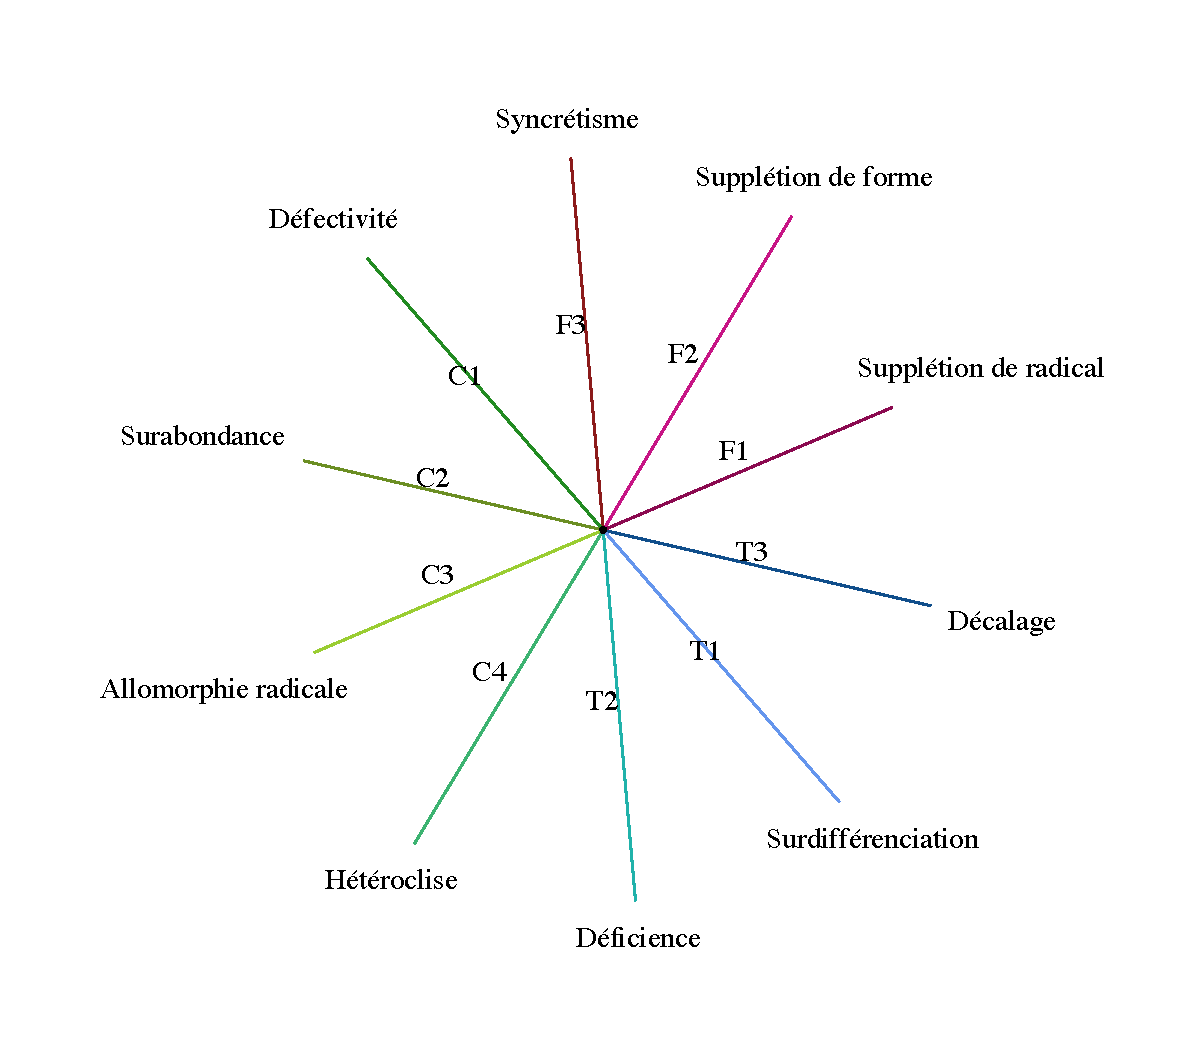
\includegraphics[height=6.4cm]{canonicityParsli}
     \end{column}
     \end{columns}

\pause
\begin{itemize}
\item[\highlighti{\danger}]\footnotesize \highlighti{Mais pas de définition pour le phénomène
  de marquage direct/inverse}
\end{itemize}
\end{frame}